\documentclass[12pt]{article}

\usepackage{amsmath}
\usepackage{graphicx}
\usepackage{subfigure}
\usepackage{float}
\usepackage{ulem}
\usepackage{bm}
\usepackage{anysize}

\marginsize{2cm}{2cm}{0.9cm}{1.8cm}

\title{CS 5200 Database Management System\\ [2ex] \begin{large} Assignment \#1 \end{large} }
\author{Jiyu Tian}
\date{}

\begin{document}
\maketitle
%%---------------------------------------------------------------
%% Question 1
%%---------------------------------------------------------------
\section{Nouns}
\textbf{User}: username, password, first name, last name, emails, phones, and addresses\\
\textbf{Faculty}: benefits, tenure status, parking, and bank account info\\
\textbf{Students}: undergrad/graduate, financial aid info, work-study, and scholarship, GPA\\
\textbf{Courses}: modules, lessons\\
\textbf{Sections}: seat capacity, instructor, teaching assistant\\
Student progress\\
\textbf{Widgets}: YouTube videos, slides, text documents, raw HTML, evaluations, etc.\\
\textbf{Evaluation widgets}: simple essay assignment, submission assignment, exam\\
\textbf{Exam}: essay, multiple choice, fill in the blank questions\\
\textbf{Semester}: fall, spring, full summer, summer 1 and summer 2\\
Registrar's office\\
\textbf{Enrollment}: the final grade, letter grade, and student feedback.\\
\textbf{Grades}: assignments, exams. 
%%---------------------------------------------------------------
%% Question 2
%%---------------------------------------------------------------
\section{Verbs}
Faculty \textbf{author} courses\\
Courses \textbf{contain} modules\\
Modules break up into lessons\\
Widgets \textbf{build} lesson\\
Exams \textbf{evaluate} student's progress\\
Registrar's office \textbf{creates} sections\\
Students \textbf{enroll in} sections\\
Registrar's office \textbf{keeps track of} student progress\\
%%---------------------------------------------------------------
%% Question 3
%%---------------------------------------------------------------
\section{Generalization/Specialization, inheritance}
Students and Faculty classes partially share the same attributes, i.e. username, password, first name, last name, emails, phones, and addresses. In Students and Faculty classes, they both have attributes which are only applicable within themselves. Therefore, Students/Faculty is a specialization with respect to User. Diagram shown in Figure \ref{gf}.
\begin{figure}[H]
\centering
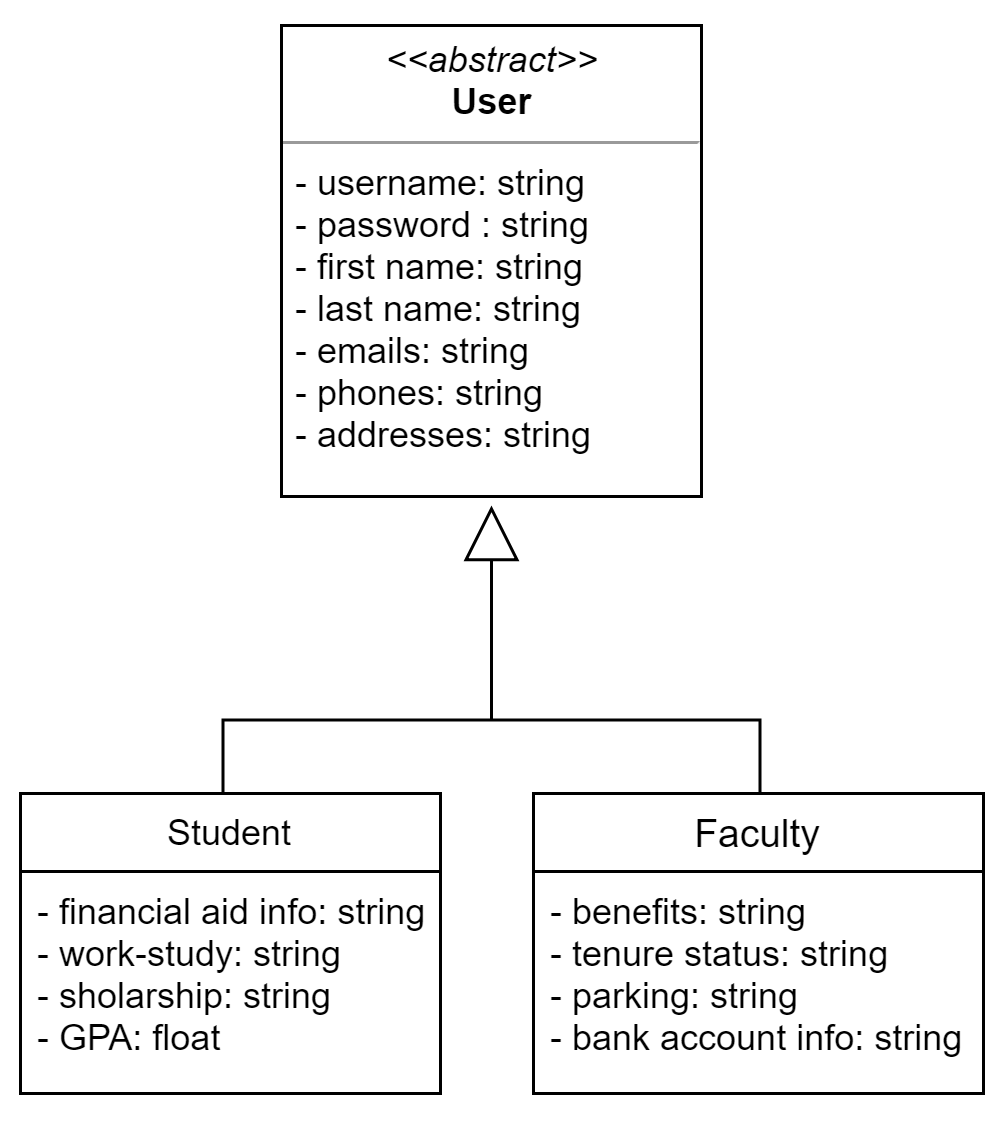
\includegraphics[width = 0.5\textwidth]{user.png}
\caption{Generalization/Specialization}
\label{gf}
\end{figure}
%%---------------------------------------------------------------
%% Question 4
%%---------------------------------------------------------------
\section{Associations, Aggregation and/or Composition}
Association is a connection between two classes. Any verb in the statement that declares a relationship can be considered as association. e.g. ``students enroll in sections'' specifies an association between student and section.\\\\
As for composition, there’s a strong lifecycle dependency between the two classes. If container is removed, so are the parts. While in aggregation, the parts can exist independently of the container. In the statement, ``courses contain modules'', ``modules contains lessons'', ``widgets build lessons'' identify several composition. Though not stated in the statement, ``registrar's office'' and ``faculty'' is aggregation. ``Registrar's office'' are composed of ``faculty'', but ``faculty'' has own lifecycle even without ``Registrar's office''.
%%---------------------------------------------------------------
%% Question 5
%%---------------------------------------------------------------
\section{Classes v.s. Attributes Analysis }
Some classes might actually be better modeled as attributes.
\begin{itemize}
    \item GPA. 
    \item instructor
\end{itemize}
Some attributes might actually be better modeled as classes.
\begin{itemize}
    \item Evaluation/Exam. Though can be listed under enumeration type of ``Widget''/``Evaluation'', it is more convenient to illustrate as class. 
    \item Grade. Easy to keep track of student progress as class.
\end{itemize}
\vfill
\clearpage
%%---------------------------------------------------------------
%% Question 6
%%---------------------------------------------------------------
\section{Data Types}
\begin{itemize}
    \item String: Most information kind of attributes could be of string type, e.g. username, password, first name, last name, emails, phones, addresses, grades, seat capacity, benefits, tenure status, parking, bank account info, etc.
    \item Int: Numerical values, e.g. year.
    \item Enum: Those with finite number of instance, e.g. questions, semester. 
\end{itemize}

%%---------------------------------------------------------------
%% Question 7
%%---------------------------------------------------------------
\section{Cardinality}
Cardinality can be derived based on statement and some common senses. e.g. ``students enroll in courses'' states a one-many relationship; ``faculty author courses'' states many-many relationship.
%%---------------------------------------------------------------
%% Question 8
%%---------------------------------------------------------------
\section{Inadequate or Redundant Relationships}
\begin{itemize}
    \item Though stated in statement that ``registrar's office creates several sections'' and ``registrar's office keeps track of student progress'', it is inadequate to draw association line between either ``registrar's office-section'' or ``registrar's office-student progess'', because there is no relationship in between.
    \item The relationship ``faculty-courses'' is redundant, because the instructor information is already stated in course's section.
    \item An one-one relationship between ``student'' and ``student progress'' is kind of redundant.
\end{itemize}
%%---------------------------------------------------------------
%% Question 9
%%---------------------------------------------------------------
\section{Reify}
\begin{itemize}
    \item Many-many relationship ``faculty-courses'' is deleted.
    \item The four-way relation ship in ``student, enrollment, section, grade'' is reified as shown in Figure \ref{rei}. The origin one is redundant, and many-many relationship between ``student'' and "section" do not readily map to relational schemas. 
\end{itemize}
\begin{figure}[H]
\centering
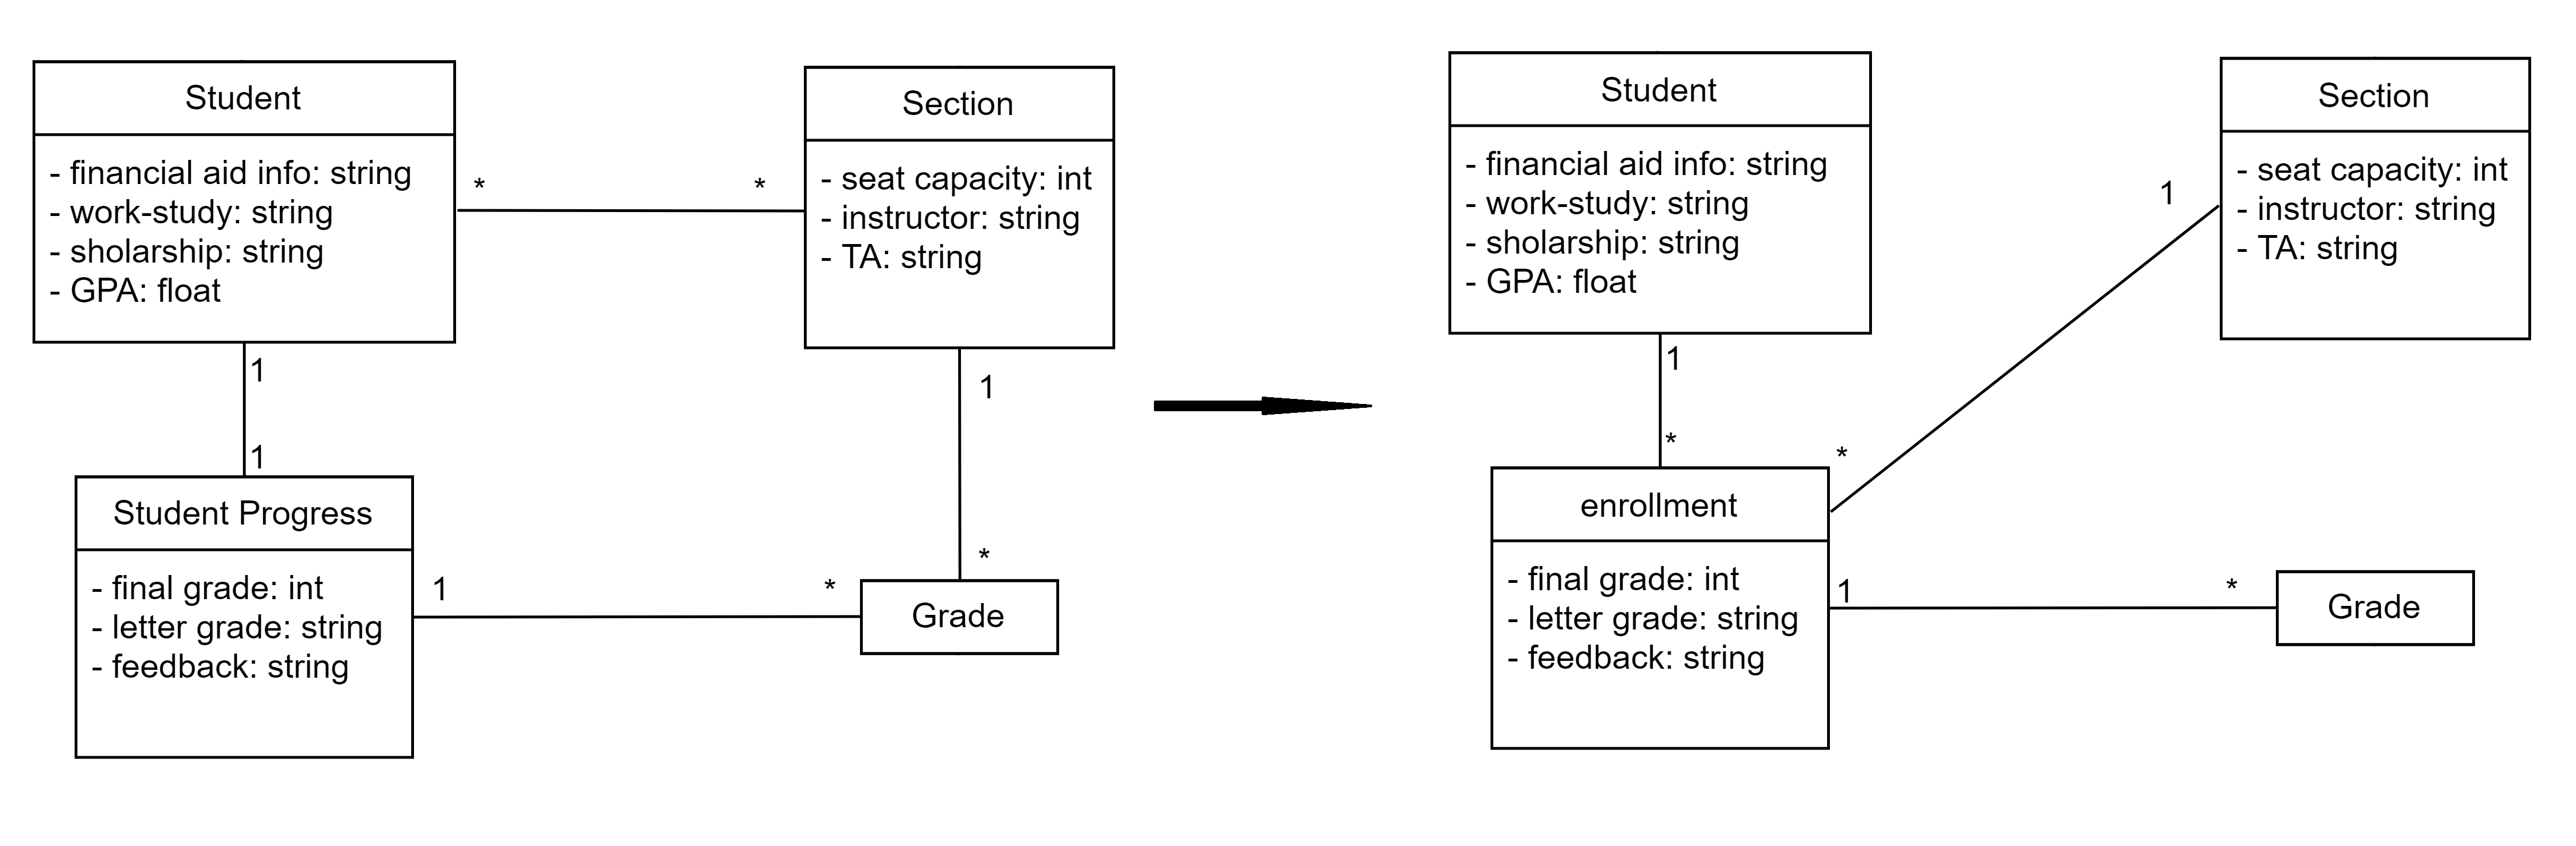
\includegraphics[width = 1\textwidth]{reify.png}
\caption{Reify}
\label{rei}
\end{figure}
\vfill
%%---------------------------------------------------------------
%% Question 10
%%---------------------------------------------------------------
% \section{Prose}


\end{document}
